% Created by tikzDevice version 0.10.1 on 2017-09-04 18:59:16
% !TEX encoding = UTF-8 Unicode
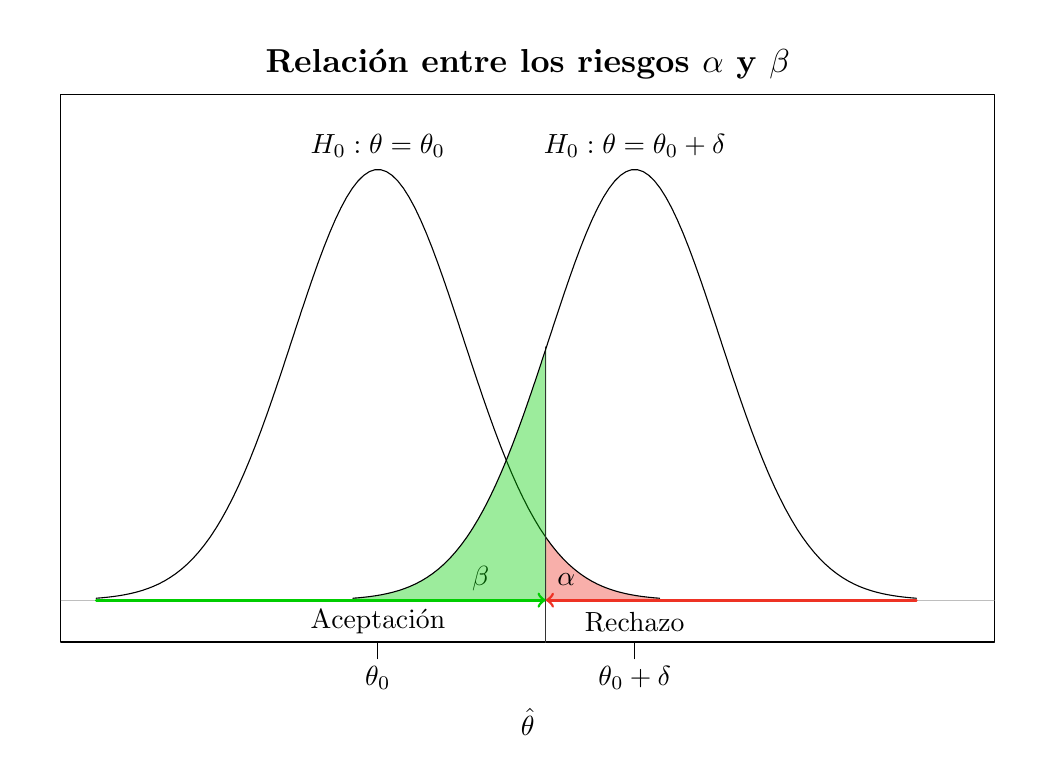
\begin{tikzpicture}[x=1pt,y=1pt]
\definecolor{fillColor}{RGB}{255,255,255}
\path[use as bounding box,fill=fillColor,fill opacity=0.00] (0,0) rectangle (361.35,258.00);
\begin{scope}
\path[clip] (  0.00,  0.00) rectangle (361.35,258.00);
\definecolor{drawColor}{RGB}{0,0,0}

\path[draw=drawColor,line width= 0.4pt,line join=round,line cap=round] ( 12.00, 36.00) --
	(349.35, 36.00) --
	(349.35,234.00) --
	( 12.00,234.00) --
	( 12.00, 36.00);
\end{scope}
\begin{scope}
\path[clip] (  0.00,  0.00) rectangle (361.35,258.00);
\definecolor{drawColor}{RGB}{0,0,0}

\node[text=drawColor,anchor=base,inner sep=0pt, outer sep=0pt, scale=  1.20] at (180.67,241.86) {\bfseries Relación entre los riesgos $\alpha$ y $\beta$};

\node[text=drawColor,anchor=base,inner sep=0pt, outer sep=0pt, scale=  1.00] at (180.67,  2.40) {$\hat\theta$};
\end{scope}
\begin{scope}
\path[clip] ( 12.00, 36.00) rectangle (349.35,234.00);
\definecolor{drawColor}{RGB}{190,190,190}

\path[draw=drawColor,line width= 0.4pt,line join=round,line cap=round] ( 12.00, 51.14) -- (349.35, 51.14);
\definecolor{fillColor}{RGB}{238,50,36}

\path[fill=fillColor,fill opacity=0.39] (187.21, 51.14) --
	(187.21, 73.87) --
	(189.27, 71.05) --
	(191.32, 68.50) --
	(193.38, 66.21) --
	(195.43, 64.16) --
	(197.49, 62.35) --
	(199.55, 60.74) --
	(201.60, 59.33) --
	(203.66, 58.09) --
	(205.72, 57.01) --
	(207.77, 56.08) --
	(209.83, 55.28) --
	(211.88, 54.59) --
	(213.94, 54.01) --
	(216.00, 53.51) --
	(218.05, 53.09) --
	(220.11, 52.74) --
	(222.16, 52.44) --
	(224.22, 52.20) --
	(226.28, 51.99) --
	(228.33, 51.83) --
	(228.33, 51.14) --
	cycle;
\definecolor{drawColor}{RGB}{0,0,0}

\path[draw=drawColor,line width= 0.4pt,line join=round,line cap=round] ( 24.77, 51.83) --
	( 26.83, 51.99) --
	( 28.89, 52.20) --
	( 30.94, 52.44) --
	( 33.00, 52.74) --
	( 35.05, 53.09) --
	( 37.11, 53.51) --
	( 39.17, 54.01) --
	( 41.22, 54.59) --
	( 43.28, 55.28) --
	( 45.33, 56.08) --
	( 47.39, 57.01) --
	( 49.45, 58.09) --
	( 51.50, 59.33) --
	( 53.56, 60.74) --
	( 55.62, 62.35) --
	( 57.67, 64.16) --
	( 59.73, 66.21) --
	( 61.78, 68.50) --
	( 63.84, 71.05) --
	( 65.90, 73.87) --
	( 67.95, 76.98) --
	( 70.01, 80.39) --
	( 72.06, 84.10) --
	( 74.12, 88.11) --
	( 76.18, 92.43) --
	( 78.23, 97.05) --
	( 80.29,101.97) --
	( 82.35,107.16) --
	( 84.40,112.61) --
	( 86.46,118.29) --
	( 88.51,124.17) --
	( 90.57,130.22) --
	( 92.63,136.40) --
	( 94.68,142.64) --
	( 96.74,148.92) --
	( 98.79,155.16) --
	(100.85,161.31) --
	(102.91,167.31) --
	(104.96,173.10) --
	(107.02,178.61) --
	(109.08,183.79) --
	(111.13,188.56) --
	(113.19,192.88) --
	(115.24,196.69) --
	(117.30,199.94) --
	(119.36,202.60) --
	(121.41,204.62) --
	(123.47,205.98) --
	(125.52,206.67) --
	(127.58,206.67) --
	(129.64,205.98) --
	(131.69,204.62) --
	(133.75,202.60) --
	(135.81,199.94) --
	(137.86,196.69) --
	(139.92,192.88) --
	(141.97,188.56) --
	(144.03,183.79) --
	(146.09,178.61) --
	(148.14,173.10) --
	(150.20,167.31) --
	(152.26,161.31) --
	(154.31,155.16) --
	(156.37,148.92) --
	(158.42,142.64) --
	(160.48,136.40) --
	(162.54,130.22) --
	(164.59,124.17) --
	(166.65,118.29) --
	(168.70,112.61) --
	(170.76,107.16) --
	(172.82,101.97) --
	(174.87, 97.05) --
	(176.93, 92.43) --
	(178.99, 88.11) --
	(181.04, 84.10) --
	(183.10, 80.39) --
	(185.15, 76.98) --
	(187.21, 73.87) --
	(189.27, 71.05) --
	(191.32, 68.50) --
	(193.38, 66.21) --
	(195.43, 64.16) --
	(197.49, 62.35) --
	(199.55, 60.74) --
	(201.60, 59.33) --
	(203.66, 58.09) --
	(205.72, 57.01) --
	(207.77, 56.08) --
	(209.83, 55.28) --
	(211.88, 54.59) --
	(213.94, 54.01) --
	(216.00, 53.51) --
	(218.05, 53.09) --
	(220.11, 52.74) --
	(222.16, 52.44) --
	(224.22, 52.20) --
	(226.28, 51.99) --
	(228.33, 51.83);

\node[text=drawColor,anchor=base,inner sep=0pt, outer sep=0pt, scale=  1.00] at (126.55,212.47) {$H_0: \theta = \theta_0$};
\end{scope}
\begin{scope}
\path[clip] (  0.00,  0.00) rectangle (361.35,258.00);
\definecolor{drawColor}{RGB}{0,0,0}

\path[draw=drawColor,line width= 0.4pt,line join=round,line cap=round] (126.55, 36.00) -- (126.55, 36.00);

\path[draw=drawColor,line width= 0.4pt,line join=round,line cap=round] (126.55, 36.00) -- (126.55, 30.00);

\node[text=drawColor,anchor=base,inner sep=0pt, outer sep=0pt, scale=  1.00] at (126.55, 20.40) {$\theta_0$};
\end{scope}
\begin{scope}
\path[clip] ( 12.00, 36.00) rectangle (349.35,234.00);
\definecolor{drawColor}{RGB}{0,0,0}

\node[text=drawColor,anchor=base,inner sep=0pt, outer sep=0pt, scale=  1.00] at (126.55, 40.86) {Aceptación};

\node[text=drawColor,anchor=base,inner sep=0pt, outer sep=0pt, scale=  1.00] at (219.33, 39.89) {Rechazo};

\node[text=drawColor,anchor=base,inner sep=0pt, outer sep=0pt, scale=  1.00] at (163.67, 56.44) {$\beta$};
\definecolor{fillColor}{RGB}{0,205,0}

\path[fill=fillColor,fill opacity=0.39] (117.55, 51.14) --
	(117.55, 51.83) --
	(119.61, 51.99) --
	(121.67, 52.20) --
	(123.72, 52.44) --
	(125.78, 52.74) --
	(127.83, 53.09) --
	(129.89, 53.51) --
	(131.95, 54.01) --
	(134.00, 54.59) --
	(136.06, 55.28) --
	(138.11, 56.08) --
	(140.17, 57.01) --
	(142.23, 58.09) --
	(144.28, 59.33) --
	(146.34, 60.74) --
	(148.40, 62.35) --
	(150.45, 64.16) --
	(152.51, 66.21) --
	(154.56, 68.50) --
	(156.62, 71.05) --
	(158.68, 73.87) --
	(160.73, 76.98) --
	(162.79, 80.39) --
	(164.85, 84.10) --
	(166.90, 88.11) --
	(168.96, 92.43) --
	(171.01, 97.05) --
	(173.07,101.97) --
	(175.13,107.16) --
	(177.18,112.61) --
	(179.24,118.29) --
	(181.29,124.17) --
	(183.35,130.22) --
	(185.41,136.40) --
	(187.46,142.64) --
	(187.46, 51.14) --
	cycle;
\definecolor{drawColor}{gray}{0.20}

\path[draw=drawColor,line width= 0.4pt,line join=round,line cap=round] (187.21, 12.13) -- (187.21,142.64);
\definecolor{drawColor}{RGB}{0,0,0}

\node[text=drawColor,anchor=base,inner sep=0pt, outer sep=0pt, scale=  1.00] at (194.59, 56.44) {$\alpha$};
\definecolor{drawColor}{RGB}{0,205,0}

\path[->, draw=drawColor,line width= 1.0pt,line join=round,line cap=round] ( 24.77, 51.14) -- (187.21, 51.14);
\definecolor{drawColor}{RGB}{238,50,36}

\path[->, draw=drawColor,line width= 1.0pt,line join=round,line cap=round] (321.11, 51.14) -- (187.21, 51.14);
\definecolor{drawColor}{RGB}{0,0,0}

\path[draw=drawColor,line width= 0.4pt,line join=round,line cap=round] (117.55, 51.83) --
	(119.61, 51.99) --
	(121.67, 52.20) --
	(123.72, 52.44) --
	(125.78, 52.74) --
	(127.83, 53.09) --
	(129.89, 53.51) --
	(131.95, 54.01) --
	(134.00, 54.59) --
	(136.06, 55.28) --
	(138.11, 56.08) --
	(140.17, 57.01) --
	(142.23, 58.09) --
	(144.28, 59.33) --
	(146.34, 60.74) --
	(148.40, 62.35) --
	(150.45, 64.16) --
	(152.51, 66.21) --
	(154.56, 68.50) --
	(156.62, 71.05) --
	(158.68, 73.87) --
	(160.73, 76.98) --
	(162.79, 80.39) --
	(164.85, 84.10) --
	(166.90, 88.11) --
	(168.96, 92.43) --
	(171.01, 97.05) --
	(173.07,101.97) --
	(175.13,107.16) --
	(177.18,112.61) --
	(179.24,118.29) --
	(181.29,124.17) --
	(183.35,130.22) --
	(185.41,136.40) --
	(187.46,142.64) --
	(189.52,148.92) --
	(191.58,155.16) --
	(193.63,161.31) --
	(195.69,167.31) --
	(197.74,173.10) --
	(199.80,178.61) --
	(201.86,183.79) --
	(203.91,188.56) --
	(205.97,192.88) --
	(208.02,196.69) --
	(210.08,199.94) --
	(212.14,202.60) --
	(214.19,204.62) --
	(216.25,205.98) --
	(218.31,206.67) --
	(220.36,206.67) --
	(222.42,205.98) --
	(224.47,204.62) --
	(226.53,202.60) --
	(228.59,199.94) --
	(230.64,196.69) --
	(232.70,192.88) --
	(234.75,188.56) --
	(236.81,183.79) --
	(238.87,178.61) --
	(240.92,173.10) --
	(242.98,167.31) --
	(245.04,161.31) --
	(247.09,155.16) --
	(249.15,148.92) --
	(251.20,142.64) --
	(253.26,136.40) --
	(255.32,130.22) --
	(257.37,124.17) --
	(259.43,118.29) --
	(261.48,112.61) --
	(263.54,107.16) --
	(265.60,101.97) --
	(267.65, 97.05) --
	(269.71, 92.43) --
	(271.77, 88.11) --
	(273.82, 84.10) --
	(275.88, 80.39) --
	(277.93, 76.98) --
	(279.99, 73.87) --
	(282.05, 71.05) --
	(284.10, 68.50) --
	(286.16, 66.21) --
	(288.22, 64.16) --
	(290.27, 62.35) --
	(292.33, 60.74) --
	(294.38, 59.33) --
	(296.44, 58.09) --
	(298.50, 57.01) --
	(300.55, 56.08) --
	(302.61, 55.28) --
	(304.66, 54.59) --
	(306.72, 54.01) --
	(308.78, 53.51) --
	(310.83, 53.09) --
	(312.89, 52.74) --
	(314.95, 52.44) --
	(317.00, 52.20) --
	(319.06, 51.99) --
	(321.11, 51.83);
\end{scope}
\begin{scope}
\path[clip] (  0.00,  0.00) rectangle (361.35,258.00);
\definecolor{drawColor}{RGB}{0,0,0}

\path[draw=drawColor,line width= 0.4pt,line join=round,line cap=round] (219.33, 36.00) -- (219.33, 36.00);

\path[draw=drawColor,line width= 0.4pt,line join=round,line cap=round] (219.33, 36.00) -- (219.33, 30.00);

\node[text=drawColor,anchor=base,inner sep=0pt, outer sep=0pt, scale=  1.00] at (219.33, 20.40) {$\theta_0+\delta$};
\end{scope}
\begin{scope}
\path[clip] ( 12.00, 36.00) rectangle (349.35,234.00);
\definecolor{drawColor}{RGB}{0,0,0}

\node[text=drawColor,anchor=base,inner sep=0pt, outer sep=0pt, scale=  1.00] at (219.33,212.47) {$H_0: \theta = \theta_0 + \delta$};
\end{scope}
\end{tikzpicture}
